\chapter{Экспериментальная часть}
 \section{Функции мобильного приложения}
 Мобильное приложение, как часть системы умного освещения, выполняет следующие функции:
\begin{description}
	\item Предоставлять имя и пароль от локальной Wi-Fi сети для следующих устройств: гирлянда, манипулятор волшебная палочка; 
	\item Отображать текущие состояние устройства гирлянда, А именно:
	отображать активно ли устройство в данный момент времени (под активностью мы понимаем наличие доступа к сети интернет у устройства) (не реализовано), отображать последний момент времени, когда устройство было активно (не реализовано), отображать, от каких манипуляторов волшебная палочка гирлянда принимает команды (не реализовано);
	\item Отображать текущие состояние устройства манипулятор волшебная палочка. А именно:
	отображать активно ли устройство в данный момент времени, отображать уровень заряда аккумулятора, отображать последний момент времени, когда устройство было активно, отображать имена WiFi сетей, к которым <<волшебная палочка>> будет автоматически подключаться при обнаружении; 
	\item Отображать ассоциации для конкретной связки устройств: гирлянда - волшебная палочка;
	\item Реализовывать возможность добавления новых ассоциаций для конкретной связки устройств;
	\item Реализовывать возможность удаления ассоциаций для конкретной связки устройств (не реализовано);
	\item Управлять гирляндой через локальную Wi-Fi сеть. А именно: иметь возможность выключить и включить гирлянду, изменить цвет свечения гирлянды на выбранный пользователем (не реализовано), переключить режим свечения гирлянды на следующий, переключить режим свечения гирлянды на заданный пользователем (не реализовано), изменить цвет свечения гирлянды на случайный, задавать в реальном времени цвет свечения каждому световому диоду гирлянды по отдельности (не реализовано);
	\item Отображать в реальном времени жесты совершаемые манипулятором волшебная палочка;
	\item Реализовывать возможность создавать новый режим свечения гирлянды (не реализовано).
\end{description}
 \section{Разработка}
 В качестве среды разработки был выбран Xcode, язык программирования - Swift. В качестве архитектурного патерна был выбран патерн сходный с <<MVP>> (схема \ref{app-sceme-naked}). А именно: файлы с кодом были разделены на следующие логические блоки:
 \begin{description}
 \item [Model] представляет из себя модель данных, а именно: объект типа класс или структура хранящий информацию о чем-либо. Прямой доступ к Model имеет только Presenter. В приложении присутствует ряд объектов типа Model, реализующие модель хранения информации о состоянии следующих устройств: гирлянда, манипулятор волшебная палочка.
 \item [View] отвечает за отображение интерфейса и обработку действий, жестов произведенных пользователем в приложении. Обменивается информацией по изменению интерфейса с Presenter. На каждый <<экран>> в приложении приходится один класс типа View.
 \item [Presenter] отвечает за взаимодействие с данными. А именно: сохранение, редактирование, удаление данных. На каждый класс типа View в приложении приходится один класс типа Presenter. 
\item [Объекты, не укладывающиеся в архитектурный патерн]В проекте присутствуют вспомогательные классы и логические блоки необходимые для запросов в сеть интернет.
 \end{description}
 Объекты Model, View, Presenter и классы для интернет запросов имеют ряд связей описанных на схеме \ref{app-sceme-naked}. Ниже представленно подробное описание связей:
  \begin{description}
  \item [View $\Rightarrow$ Presenter] Класс View держит сильной ссылкой класс Presenter. Через эту связь View передает информацию о совершаемых пользователем действиях в Presenter.
  \item [Presenter $\Rightarrow$ Model] Класс Presenter держит сильной ссылкой класс Model. Через эту связь Presenter инициирует изменение переменных и других объектов класса Model.
  \item [Model $\Rightarrow$ Network] Класс Model держит сильной ссылкой класс, отвечающий за запросы в интернет. Через эту связь класс Model обновляет свои переменные и другие объекты, а также инициирует различные процессы в системе освещения - например, включение гирлянды.
  \item [Model $\Rightarrow$ Presenter] Класс Model держит слабой ссылкой класс Presenter. Через эту связь класс Model уведомляет Presenter об успешном совершении интернет запроса или об изменении своих переменных и других объектов.
  \item [Presenter $\Rightarrow$ View] Класс Presenter держит слабой ссылкой класс View. Через эту связь Presenter инициирует изменение визуальных объектов.
   \end{description}
 \begin{figure}[ht]
   \centering
   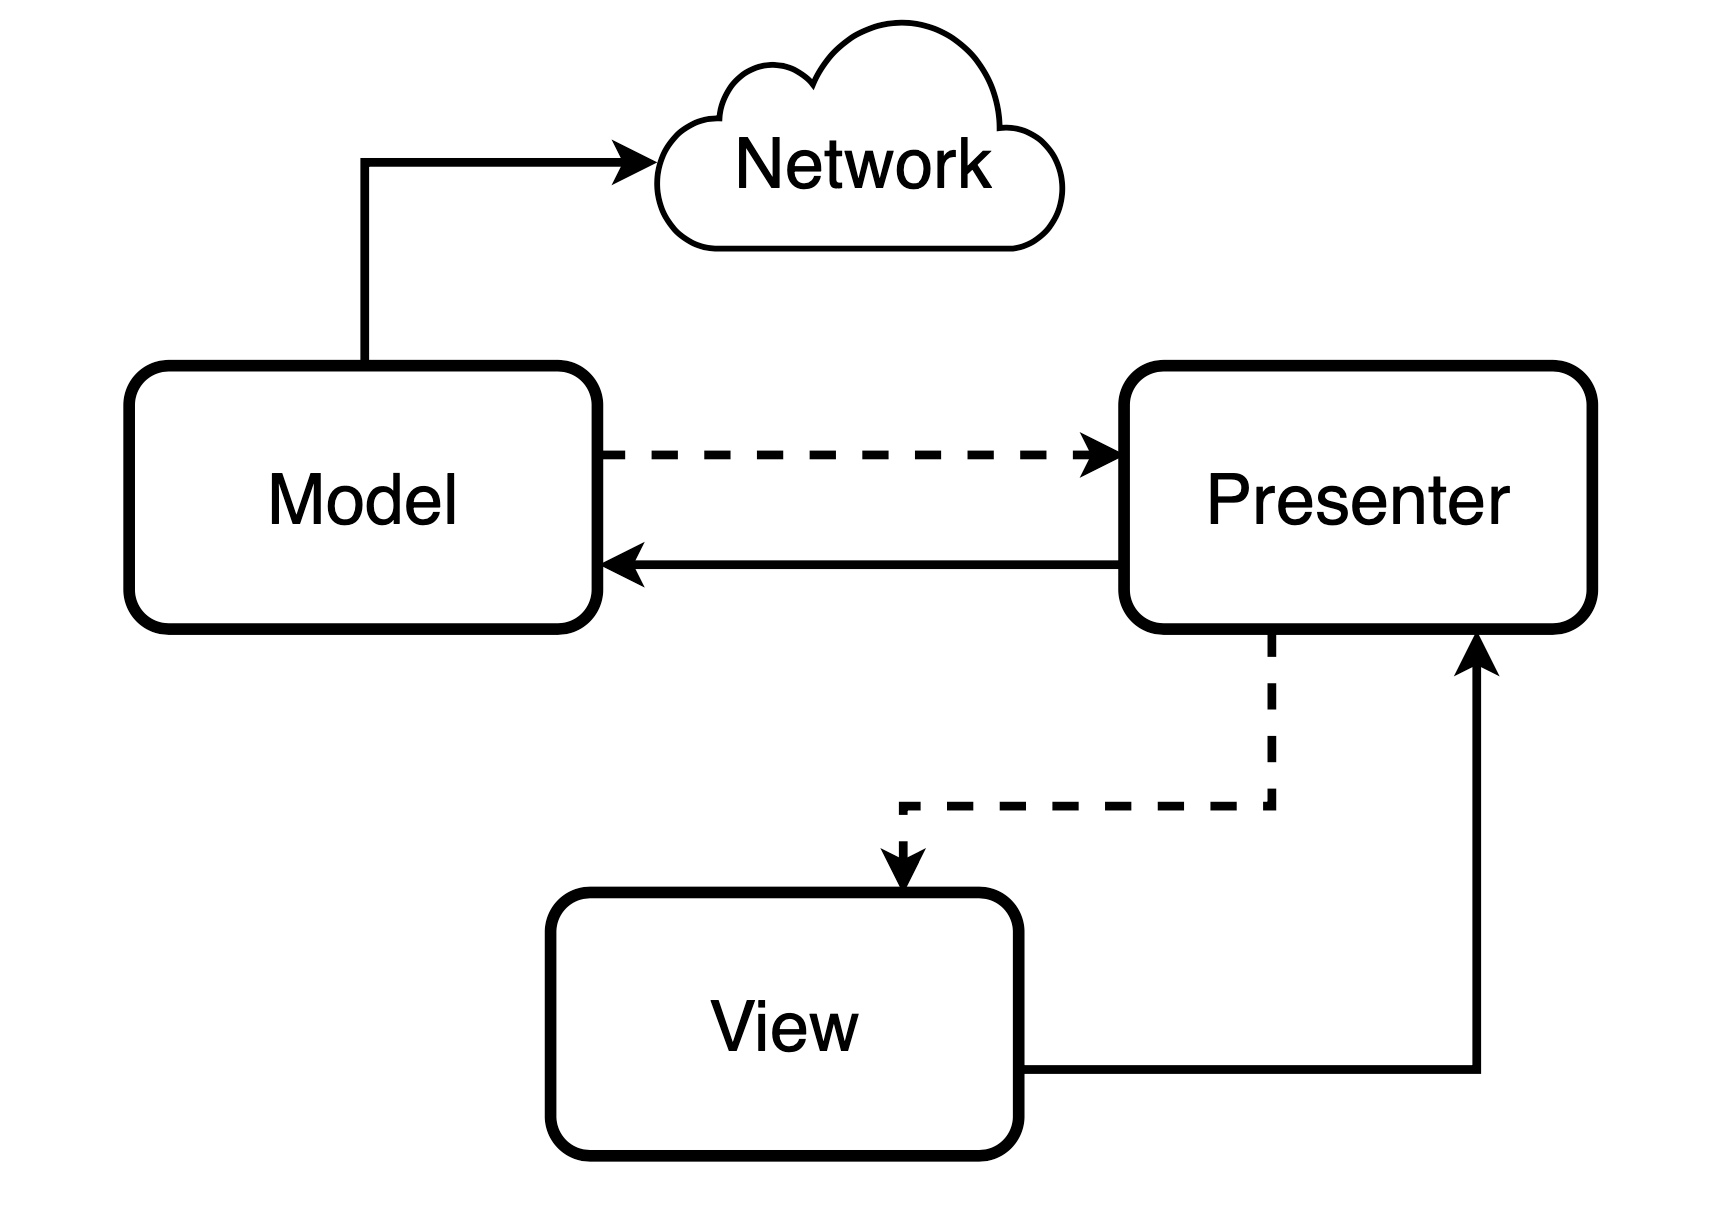
\includegraphics[scale=.25]{figures/mvp.jpg}
    \caption{Архитектурный патерн MVP}
    \label{mvp}
\end{figure}
  \section{Результат}
  Результат разработки описывается иерархией представлений (экранов) мобильного преложения (схема \ref{app-sceme-naked}).
  \begin{description}
  \item [Представление 1.1] Начальный экран, появляется сразу после открытия приложения. Содержит список устройств, а именно список гирлянд и манипуляторов <<волшебная палочка>>, которым был предоставлен доступ к локальному Wi-Fi. Также содержит кнопку <<Add new device>>, открывающую экран 2.1.
  \item [Представление 1.2] Экран настроек, пуст в текущей реализации.
  \item [Представление 2.1] Экран, содержащий элементы по управлению гирляндой. А именно:
  \begin{enumerate} 
    \item Переключатель для включения/выключения гирлянды
    \item Кнопка <<Switch mode>> меняющая режим свечения гирлянды на следующий
    \item Кнопка <<Random color>> меняющая цвет свечения гирлянды на случайный
\end{enumerate}
  \item [Представление 2.2] Экран для добавления нового устройства в список экрана 1.1. Имеет список устройств, доступных для добавления.
  \item [Представление 2.3] Экран, содержащий информацию о волшебной палочке в виде таблицы. А именно, таблица содержит следующие ячейки:
%   \renewcommand{\labelenumii}{\arabic{enumi}.\arabic{enumii}.}
\begin{enumerate} 
    \item Ячейка, отображающая активна ли волшебная палочка в данный момент
    \item Ячейка, отображающая насколько давно волшебная палочка была в сети
    \item Ячейка, отображающая уровень заряда аккумулятора
    \item Ячейка, отображающая список имен известных Wi-Fi сетей
   
    \item Ячейка, открывающая экран ассоциаций при нажатии
    \item Ячейка, открывающая экран жестов при нажатии
\end{enumerate}
Также содержит кнопку <<Update>>, обновляющую информацию в ячейках, описанных выше.
  \item [Представление 3.1] Экран, содержащий инструкцию по добавлению нового устройства. Отображает прогресс пользователя по выполнению инструкции.
    \item [Представление 3.2] Экран, содержащий ассоциации имеющиеся для данной волшебной палочки. Также содержит кнопку <<Add>>, открывающую экран 4.1.
    \item [Представление 3.3] Экран, в реальном времени отображающий жесты совершаемые волшебной палочкой.
    \item [Представление 4.1] Экран, реализующий создание новой ассоциации. Содержит меню выбора соответствий между жестом и действием. Также содержит кнопку <<Add>>, которая возвращает на экран 3.1. 
 \end{description}
 Имеются переходы между экранами в иерархии:
  \begin{description}
  \item [Переход 1.1 - 1.2] Осуществляется нажатием на правую часть меню в нижней части экрана (этот элемент имеет название tab bar). Так как tab bar доступен на всех экранах в иерархии, то и переход в настройки и обратно доступен везде. Таким образом помимо перехода 1.1 - 1.2, существуют аналогичные переходы: 1.2 - 1.1, 2.1 - 1.2, 1.2 - 2.1, 2.2 - 1.2 и тд. 
  \item [Переход 1.1 - 2.1] Осуществляется нажатием на ячейку типа <<гирлянда>> из списка доступных устройств.
  \item [Переход 1.1 - 2.2] Осуществляется нажатием на кнопку <<Add new device>> в верхней правой части
  \item [Переход 1.1 - 2.3] Осуществляется нажатием на ячейку типа <<волшебная палочка>> из списка доступных устройств.
  \item [Переход 2.2 - 3.1] Осуществляется нажатием на элемент типа <<гирлянда>> или типа <<волшебная палочка>> из списка устройств для добавления.
  \item [Переход 2.3 - 3.2] Осуществляется нажатием на ячейку ассоциаций - <<Associations>>.
  \item [Переход 2.3 - 3.3] Осуществляется нажатием на ячейку жестов - <<Moves>>.
  \item [Переход 3.1 - 1.1] Осуществляется автоматически после успешного выполнения пользователем всех пунктов инструкции. После выполнения перехода на экране 1.1 появляется только что добавленное устройсво.
  \item [Переход 3.2 - 4.1] Осуществляется нажатием на кнопку <<Add>> в верхней правой части.
  \item [Переход 4.1 - 3.2] Осуществляется нажатием на кнопку <<Add>> в верхней правой части. После выполнения перехода на экране 3.2 появляется только что созданная ассоциация.
  \item [Переходы навигации] На всех экранах второго и более уровней в иерархии представлений существует возможность вернуться на экран ниже, нажав на кнопку расположенную в верхней левой части экрана. Таким образом, все переходы, ведущие по иерархии вверх, обратимы. 
 \end{description}
\begin{figure}[ht]
   \centering
   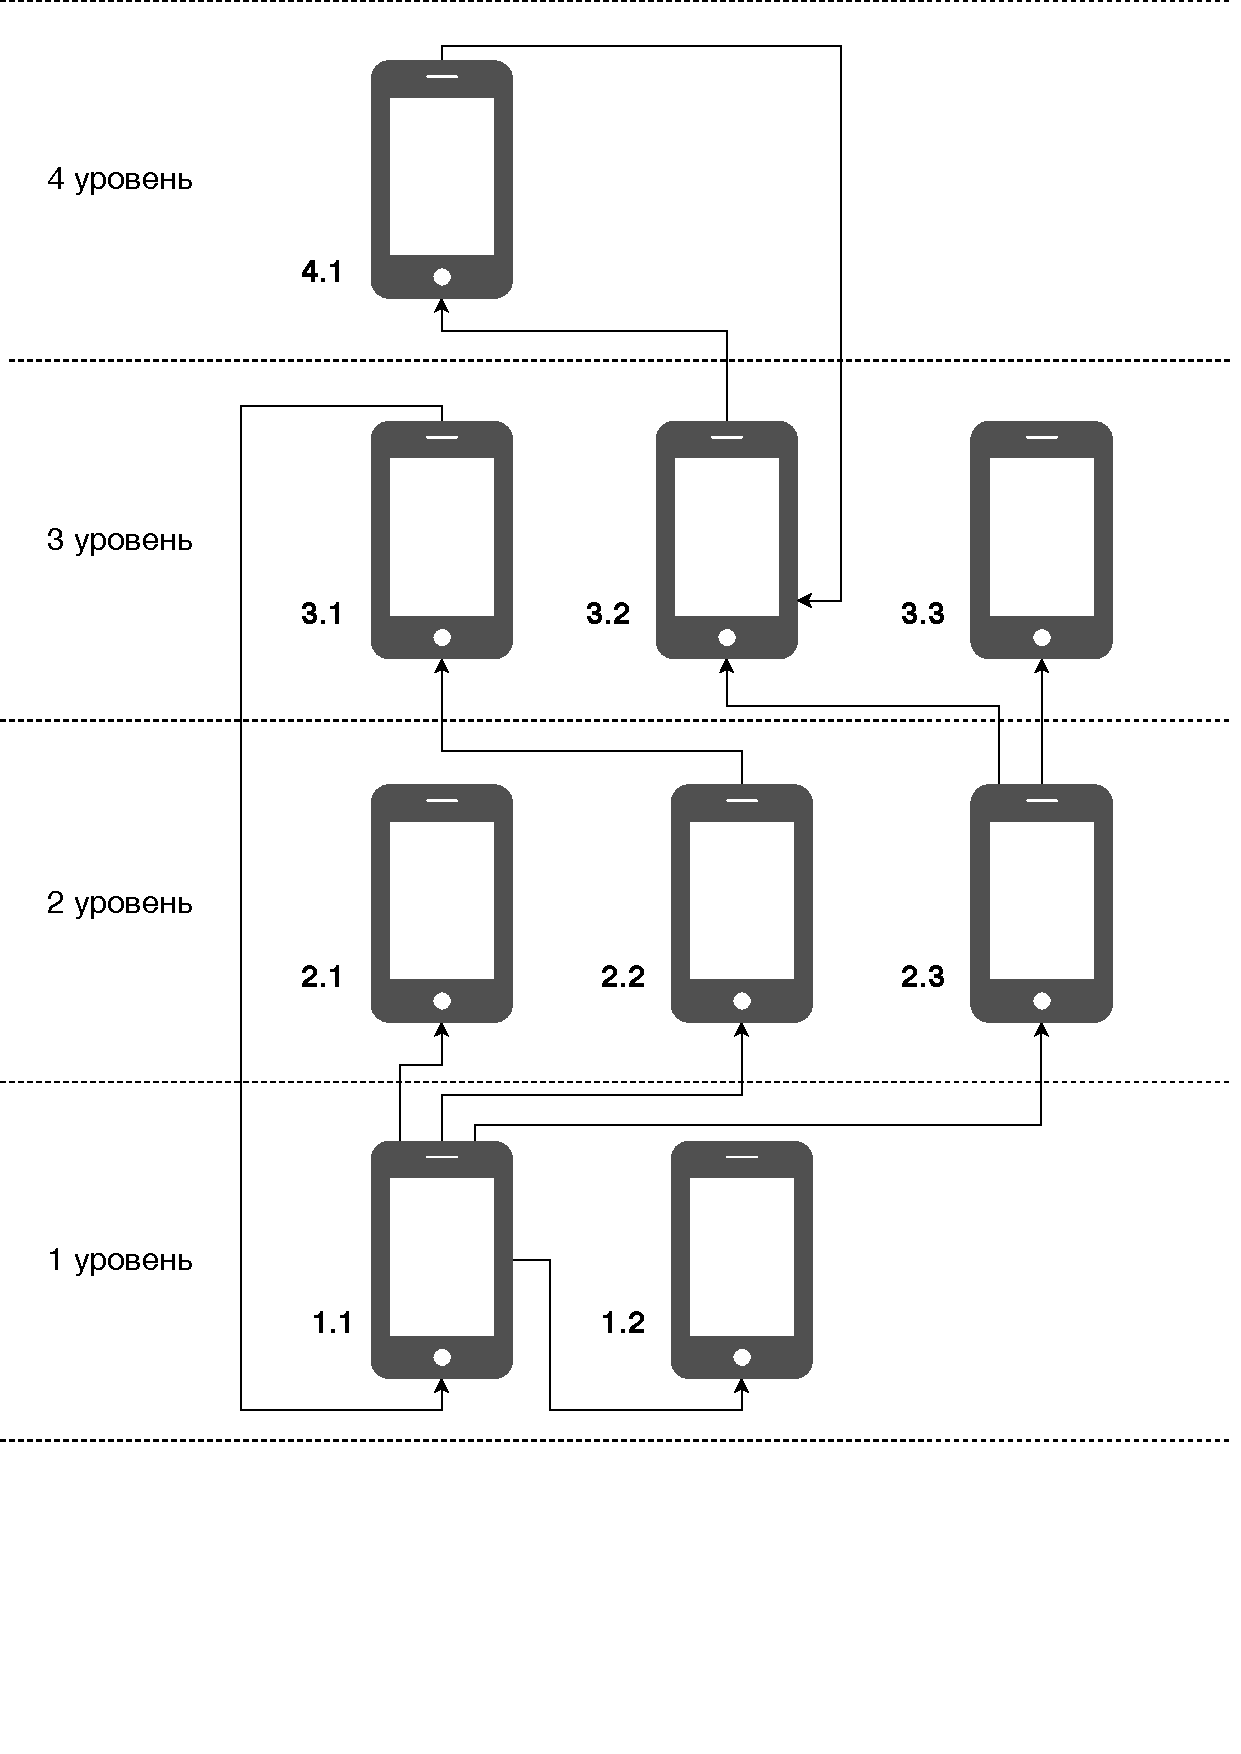
\includegraphics[scale=.75]{figures/app-sceme-naked.pdf}
    \caption{Иерархия представлений (экранов) в мобильном приложении}
    \label{app-sceme-naked}
\end{figure}
\label{cha:Experiment}
 